\documentclass[12pt]{article}
\usepackage[top=0.9in, bottom=0.9in, left=0.9in, right=1.1in]{geometry}

\usepackage{graphicx,color,enumitem}
\usepackage{amsmath,amsthm,amsbsy}
\usepackage{palatino}

%% Setup aproblem environment, 
%% aproblem items
%% subproblems environment
%% subproblem items
\makeatletter
\newcounter{probcount}
\newcounter{subprobcount}
\newlength\probsep
\newlength\pshrinking
\newif\iffirstprob
\newenvironment{aproblems}%
  {\ifhmode\unskip\par\fi\setcounter{probcount}{0}\probsep\parskip
  \sbox\@tempboxa{\textbf{9.}}\pshrinking\wd\@tempboxa\advance\pshrinking\labelsep
  \let\hproblem\aproblem
  \advance\linewidth -\pshrinking
  \advance\@totalleftmargin\pshrinking
  \advance\leftskip\pshrinking}%
  {\ifhmode\unskip \par\fi\advance\leftskip-\pshrinking}%

\newcommand{\aproblem}{%
  \setcounter{subprobcount}{0}%
  \stepcounter{probcount}%
  \def\@currentlabel{\arabic{probcount}}%
  \ifhmode
    \unskip \par
  \fi
%  \addpenalty{-4000}%
  \iffirstprob\else\addvspace\probsep\fi
  \firstprobfalse
  \hskip -\labelwidth\hskip -\labelsep 
  \hbox to\labelwidth{\hss\textbf{\arabic{probcount}.}}\hskip\labelsep
}%

\newcommand{\subprob}{\item\def\@currentlabel{\arabic{probcount}\alph{\thelistlabel}}}
\newcommand{\skipproblem}{\stepcounter{probcount}}


%% The following commands put defined left and right headers on the top, and a page number
%% on the bottom of all pages beyond page 1
\usepackage{fancyhdr}
\pagestyle{fancy}
\fancyfoot[C]{\ifnum \value{page} > 1\relax\thepage\fi}
\fancyhead[L]{\ifx\@doclabel\@empty\else\@doclabel\fi}
\fancyhead[R]{\ifx\@docdate\@empty\else\@docdate\fi}
\headheight 15pt
\def\doclabel#1{\gdef\@doclabel{#1}}
\def\docdate#1{\gdef\@docdate{#1}}
\makeatother

%% General formatting parameters
\parindent 0pt
\parskip 6pt plus 1pt


\doclabel{Math F251: Section 4.1 Worksheet}
\docdate{Monday 22 October 2018}


\begin{document}
\renewcommand{\d}{\displaystyle}

\begin{aproblems}
% 4.1 #5
\aproblem  Use the graph to state the absolute and local maximum and minimum values of the function.

\hfill 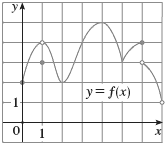
\includegraphics[width=0.3\textwidth]{4p1-5}

\vspace{0.5in}

% 4.1 #22 with small mod
\aproblem  Sketch the graph $f$ by hand and use your sketch to find the absolute and local maximum and minimum values of $f$.
$$f(t) = \cos(t), \quad -\frac{3\pi}{2} \le t < \pi \hspace{4.0in}$$

\vfill

% 4.1 #10
\aproblem  Sketch a graph of a function $f$ which is continuous on $[1,5]$, which has an absolute maximum at $2$, has an absolute minimum at $5$, and for which $4$ is a critical number but neither a local maximum nor local minimum.

\vfill

\clearpage
\newpage
\thispagestyle{plain}

% 4.1 #49
\aproblem  Find the absolute maximum and minimum values of $f$ on the given interval:
    $$f(x) = 2 x^3 - 3 x^2 - 12 x + 1, \qquad [-2,3] \hspace{3.8in}$$

\vfill

% 4.1 #59
\aproblem  Find the absolute maximum and minimum values of $f$ on the given interval:
    $$f(x) = x^{-2} \ln x, \qquad [\tfrac{1}{2},4] \hspace{4.0in}$$

\vfill

% 4.1 #36
\aproblem  Find the critical numbers of the function:
    $$h(p) = \frac{p-1}{p^2+4} \hspace{4.5in}$$

\vfill

\end{aproblems}

\end{document}
